\documentclass[xetex,mathserif,serif]{beamer}

\usepackage{mathspec}
\usepackage{xltxtra,fontspec,xunicode}
\usepackage{listings}

% Features
\setbeamertemplate{navigation symbols}{}

% Fonts
\setmainfont{Helvetica}
\setmathsfont(Digits,Latin,Greek){Helvetica}
\setmonofont{Monaco}

\title{The State of Haskell, 2011 survey results}
\author{Johan Tibell\\johan.tibell@gmail.com}
\date{2011-09-22}

\begin{document}

\frame{\titlepage}

\begin{frame}
  \frametitle{The State of Haskell, 2011 Survey}
  \begin{itemize}
  \item I run a yearly Haskell user survey
  \item Good source of information for current problems, as
    experienced by the ``average'' Haskell user
  \item I will focus on one main theme
  \end{itemize}
\end{frame}

\begin{frame}
  \frametitle{Performance of Haskell code}
  \begin{center}
  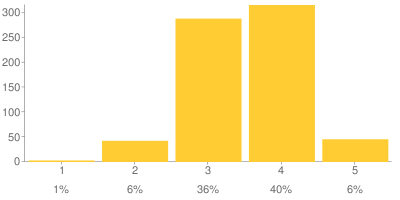
\includegraphics[width=\textwidth]{performance}
  \end{center}
  Scale: 1 - poor, 5 - excellent
\end{frame}

\begin{frame}
  \frametitle{Ease of reasoning about performance}
  \begin{center}
  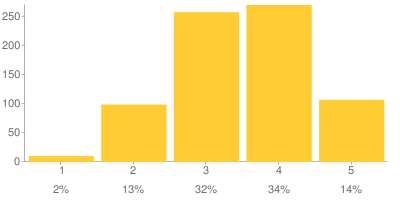
\includegraphics[width=\textwidth]{reasoning}
  \end{center}
  Scale: 1 - easy, 5 - hard
\end{frame}

\begin{frame}
  \frametitle{The working Haskell engineer}
  \begin{itemize}
  \item Predictable performance is important to engineers because...
  \item ...not knowing if you will be able to solve a future
    (performance) problem in the program that pays your bills is
    scary!
  \end{itemize}
\end{frame}

\begin{frame}
  \frametitle{Dirty talk}
  \begin{itemize}
  \item \textbf{Reasoning about performance in Haskell is possible}: a
    small group of people know how to
  \item Talking about performance/operational reasoning is considered
    ``dirty'': \textbf{we don't teach people how to do it}
  \end{itemize}
\end{frame}

\begin{frame}
  \frametitle{Conclusion/Call-to-action}
  What I think we should do:
  \begin{enumerate}
  \item Pay the issues some attention
  \item Figure out how to teach performance reasoning:
    \begin{itemize}
    \item When is the right time to introduce the topic?
    \item What do you teach first, second, etc?
    \end{itemize}
  \end{enumerate}
\end{frame}

\end{document}

%%% Local Variables:
%%% mode: latex
%%% TeX-master: t
%%% TeX-PDF-mode: t
%%% End:
